% Document type with options
\documentclass[fleqn,letterpaper,12pt]{report}

% Required packages and settings (DO NOT UPDATE THIS)
\usepackage{UN5390}
../LaTeXTemplates/Course/UN5390_Settings.tex

% Assignment-specific setting (UPDATE THIS WHEN NECESSARY)
\week{07}

% Document begins
\begin{document}

% Title (DO NOT UPDATE THIS)
\assignmenttitle

%
\phantomsection
\addcontentsline{toc}{section}{Problem \# 1}
\problem
Augusta Ada King-Noel, Countess of Lovelace (née Byron; 10 December,1815 $-$ 27 November,1852) was an English mathematician and writer, chiefly known for her work on Charles Babbage's early mechanical general-purpose computer, the Analytical Engine.

She was the daughter of poet George, Lord Byron.Her educational and social exploits brought her into contact with scientists such as Andrew Crosse, Sir David Brewster, Charles Wheatstone, Michael Faraday and the author Charles Dickens, which she used to further her education. Ada described her approach as ``poetical science" and herself as an ``Analyst (and Metaphysician)".

Lovelace became close friends with her tutor Mary Somerville, who introduced her to Charles Babbage in 1833.During a nine-month period in 1842$-$43, Lovelace translated the Italian mathematician Luigi Menabrea's article on Babbage's newest proposed machine, the Analytical Engine. With the article, she appended a set of notes Explaining the Analytical Engine's function was a difficult task, as even many other scientists did not really grasp the concept and the British establishment was uninterested in it, Lovelace's notes even had to explain how the Analytical Engine differed from the original Difference Engine Her work was well received at the time; the scientist Michael Faraday described himself as a supporter of her writing.

Second Tuesday of October is celebrated as Ada Lovelace Day(ALD) in honor of her contributions.The date is arbitrary, chosen in an attempt to make the day maximally convenient for the most number of people avoiding major public holidays, school holidays, exam season, and times of the year when people might be hibernating.Ada was born on 10 December and, in the UK where Ada Lovelace Day is based, December is swamped by Christmas parties, making venue hire tricky. Given her tragically early death at the age of 36, it would feel inappropriate to celebrate her deathday on 27 November.\cite{ll}

Ada Lovelace is known for the Algorithm that could compute Bernoulli numbers which was considered by many as the first computer program in the history of mankind, making her the first computer programer.

The function is given as,
\begin{equation}
\begin{split}	
	0\,=\, -\frac{1}{2}.\frac{2n-1}{2n+1}\,+\,B_1\left(\frac{2n}{2}\right)\,+\,B_3\left(\frac{2n.(2n-1).(2n-1)}{2.3.4}\right)\,+\,B_5\left(\frac{2n.(2n-1).(2n-4)}{2.3.4.5.6}\right)\\
	\,+..+\,B_{2n-1}
	\end{split}
\end{equation}
where $B_1$, $B_3$, $B_5$ are the Bernouli's numbers. 
The above equation can be written in general form as ,
\begin{equation}
	0\,=\,A_0+ A_1B_1 + A_2B_2 + A_3B_3 + A_5B_5 
	+...+ B_{2n-1}
\end{equation}

So the strategy could be used to calculate Bernoulli's numbers recursively. The first few numbers are,

$$ B_2 = \frac{1}{6}, B_4 = \frac{-1}{30}, B_6 = \frac{-1}{42}$$

The Machine that used the Algorithm(Analytical Engine) could compute $B_{2n}$ as long as it could store all the previous numbers of Bernoulli.\cite{lll}
%
\newpage
\phantomsection
\addcontentsline{toc}{section}{Problem \# 2}
\problem
Vo2max is the maximum oxygen consumption [$mL/(kg.min)$]. By Daniels and Gilbert formula Vo2max can be calculated and subsequently given a Distance($S$) and Vo2max, we can predict the time by numerical methods as given in the program {\tt vo2max.m}. Velocity{($v$)} required in the formula is calcuated as {$S/t$} where {$ t $} is the time. The table is completed as follows:
% Please add the following required packages to your document preamble:
% \usepackage{graphicx}
\begin{table}[h]
\centering
\caption{Time given Vo2Max and Distance}
\label{my-label}
\begin{tabular}{|l|l|l|l|l|}
\hline
$d(miles)$ & $t(h:mm:ss)$ & $VO_2Max$  & $t_c(h:mm:ss)$ & $e = |t - t_c|$ \\ \hline \hline
3.10       & 00:22:07    & {\tt43.829318} & {\tt00:22:07}      & {\tt0}               \\ \hline
6.20       & 0:47:47     & {\tt41.776160} & {\tt00:47:47}      & {\tt0}               \\ \hline
13.10      & 1:43:02     & {\tt43.231491} & {\tt1:43:02}       & {\tt0}               \\ \hline
26.20      & 4:06:21     & {\tt36.411280} & {\tt4:06:21}       & {\tt0}               \\ \hline
\end{tabular}%
\end{table}

The Program that generated the outputs in the table is named \textcolor{Green}{\tt vo2max.m}
%
\newpage
\phantomsection
\addcontentsline{toc}{section}{Problem \# 3}
\problem
Newton's law of cooling states that the rate of heat loss of a body is proportional to the difference in temperatures between the body and its surrounding environment which can be written as,
\begin{equation}
$$\frac{dT}{dt} = k(T_{room} -T)$$
\end{equation}

,where $t$ is the time at that instance, $T$ is the temperature of the liquid at that instance $k$ is a constant.

With assumptions that the temperature of the room remains constant and also assuming discrete time($mins$) steps $\Delta t = 1$. 
\begin{equation}
$$\frac{1}{T_{room}-T} = kdt$$
\end{equation}

Integrating on both sides, we get,
\begin{equation}
$$log|T_{room}-T| = kt+c$$
\end{equation}
\begin{equation}
$$e^{log|T_{room}-T|} = e^{kt+c}$$
\end{equation}
\begin{equation}
$$|T_{room}-T| = C.e^{kt}$$
\end{equation}
,where $C = e^c$.
\begin{equation}
$$T = T_{room} - C.e^{kt}$$
\label{PQ2_EQ1}
\end{equation}

$C$ can be easily found by using the initial conditions i.e at $t=0$
thus,
$C = T_{room}-T$
which is $70-200 = -130$ in this problem.

Substituting the above in \eqref{PQ2_EQ1}, we have the Equation,
\begin{equation}
$$T = T_{room} - 130.e^{kt}$$
\end{equation}

For discrete time, this equation can be written as 
\begin{equation}
T_{n+1} = T_{n} + k(T_{room} - T_n)\Delta t
\end{equation}
which can further be written as 
\begin{equation}
$$T_{n+1} = \alpha T_{n} + \beta\Delta t\;\;$$
\label{EQ2}
\mbox{,where $\alpha = 1 - k\Delta t$ and $\beta = k\Delta tT_{room}$}
\end{equation}

Using \eqref{EQ2}, the Temperature and the time required for the liquid to reach the room temperature within in a error margin of $0.1^oF$. The program is in the file named \tt{\textcolor{Green}{problem3.m}
\begin{figure}[ht!]
	\centering
	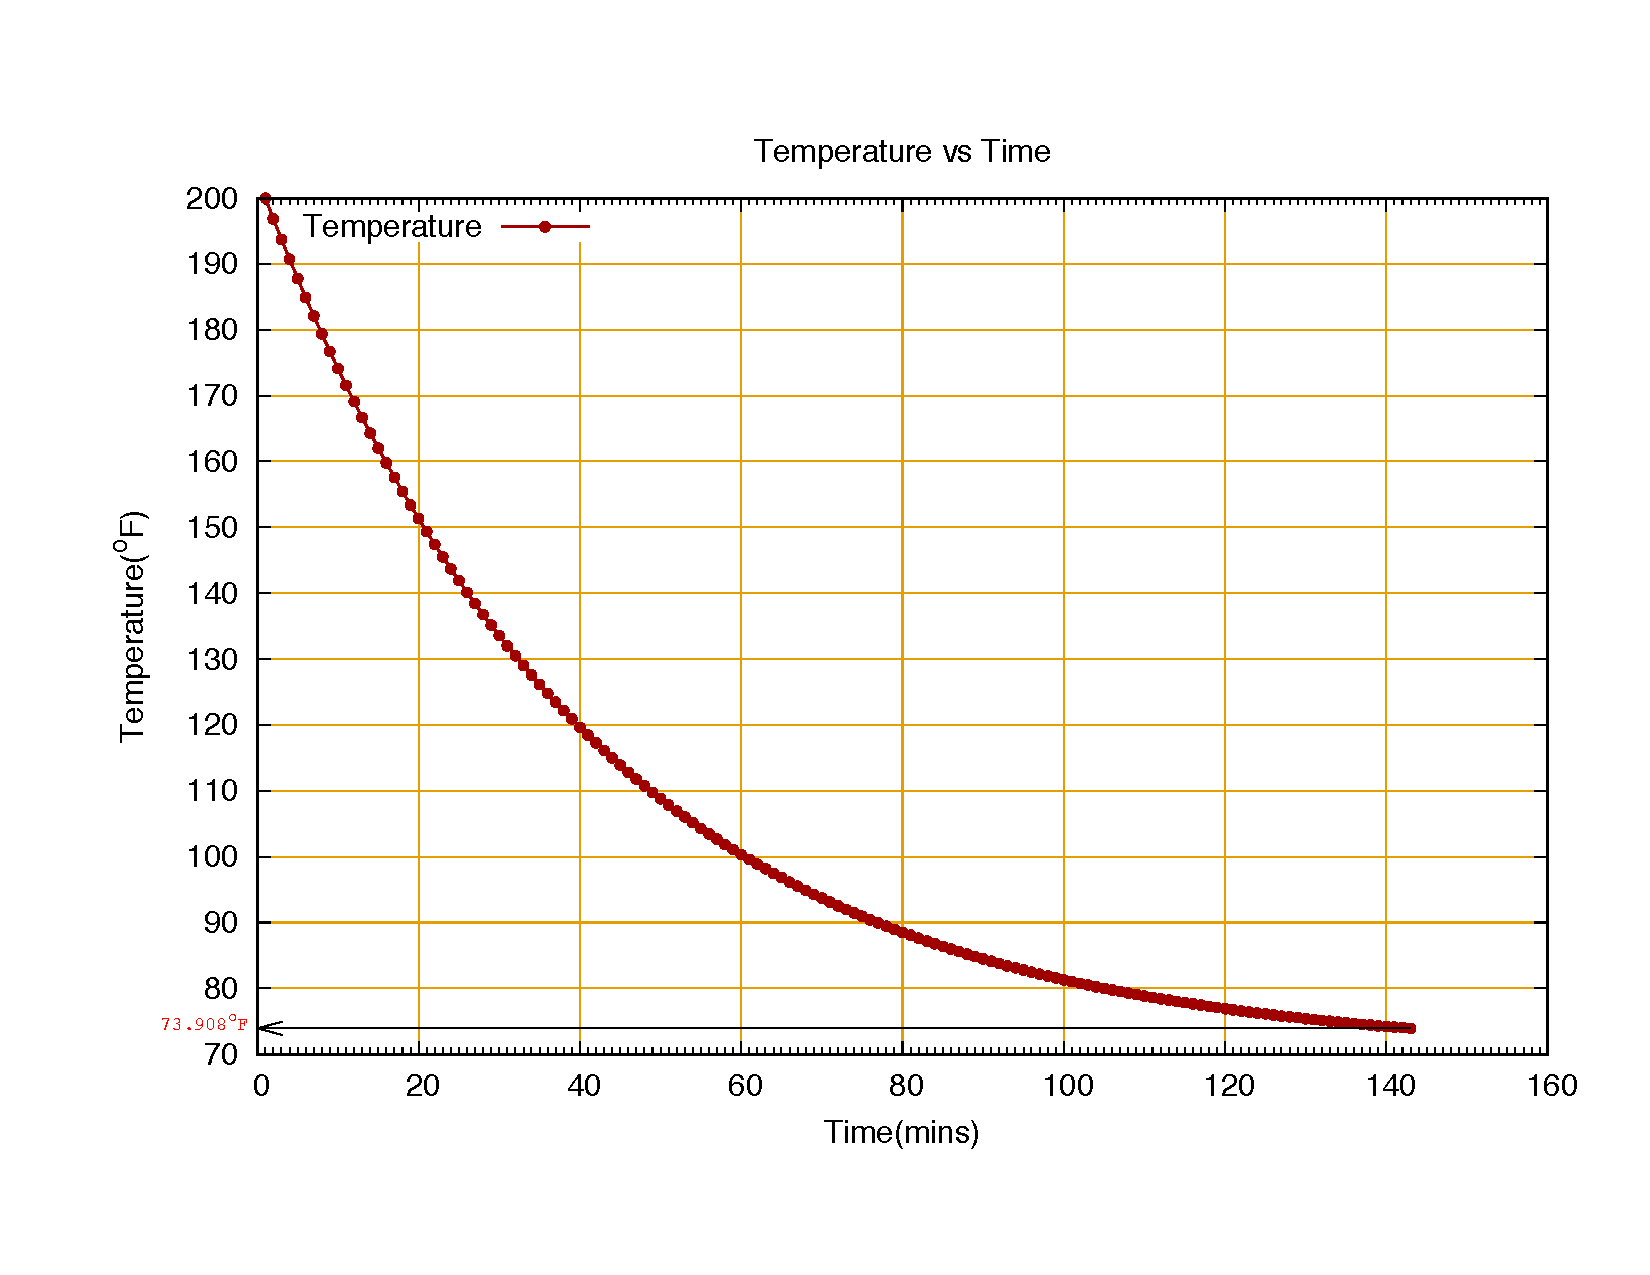
\includegraphics[height=120mm,width=160mm]{T.pdf}
	\caption{Rate of change of Temperature of the liquid w.r.t Time\label{overflow}}
\end{figure}

\newpage
\phantomsection
\addcontentsline{toc}{section}{Problem \# 4}
\problem
\newpage
% References
% http://tex.stackexchange.com/questions/84099/bibliographies-from-multiple-bib-files
\phantomsection
\addcontentsline{toc}{section}{References}
\section*{References}
\bibliographystyle{unsrt}
\bibliography{sgowtham,slanka} % REPLACE john WITH YOUR MICHIGAN TECH ISO USERNAME

% Document ends
\end{document}
